\documentclass{article}
\usepackage[margin=0.5in]{geometry}
\usepackage[utf8]{inputenc}
\usepackage{pgfplots}
\pgfplotsset{width=10cm,compat=1.9}
\begin{document}

                            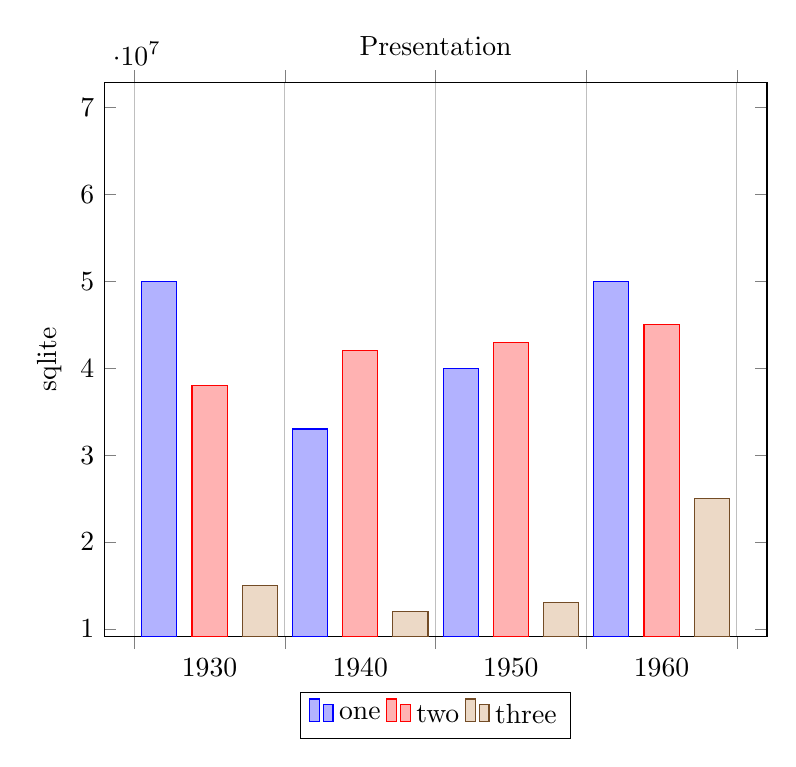
\begin{tikzpicture}
                            \begin{axis}[
                            x tick label style={/pgf/number format/1000 sep=},
                            ylabel=sqlite,
                            xlabel=sql,
                            enlargelimits = 0.050000,
                            legend style={at={(0.500000,-0.100000)},	anchor=north, legend columns=-1},
                            ybar interval=0.700000,
                            title={Presentation}
                            ]
                            \addplot
	coordinates {(1930,50e6) (1940,33e6)
		 (1950,40e6) (1960,50e6) (1970,70e6)};

\addplot
	coordinates {(1930,38e6) (1940,42e6)
		(1950,43e6) (1960,45e6) (1970,65e6)};

\addplot
	coordinates {(1930,15e6) (1940,12e6)
		(1950,13e6) (1960,25e6) (1970,35e6)};

\legend{one,two,three}
                            \end{axis}
                            \end{tikzpicture}
											\hskip 5pt
\begin{tikzpicture}
                            \begin{axis}[
                            title={Production},
                            xlabel={Cost},
                            ylabel={Year},
                            xmin=0, xmax=12,
                            ymin=0, ymax=11,
                            xtick={0, 2, 4, 6, 8, 10, 12},
                            ytick={0, 2, 4, 6, 8, 10, 11},
                            legend pos=north,
                            ymajorgrids=true,
                            grid style=dotted,
                            ]
                            \addplot[
                            dashed, color=red, mark=diamond, mark options={scale=2}
                            ]
                            coordinates {
                            (2,1)(4,3)(6,9)(8,7)(10,9)
                            };
\addplot[
                            , color=blue, mark=square, mark options={scale=2}
                            ]
                            coordinates {
                            (2,2)(4,1)(6,3)(8,7)(2,10)
                            };

                            \legend{Saurabh, Topcoder}
                            \end{axis}
                            \end{tikzpicture}
											\hskip 5pt
\begin{tikzpicture}
                    \begin{axis}[
                    title={Production},
                    xlabel={Cost},
                    ylabel={Year},
                    xmin=0, xmax=12,
                    ymin=0, ymax=11,
                    xtick={0, 2, 4, 6, 8, 10, 12},
                    ytick={0, 2, 4, 6, 8, 10, 11},
                    legend pos=north,
                    ymajorgrids=true,
                    grid style=dotted,
                    ]
                    \addplot[
                        dashed, color=red, mark=diamond, mark options={scale=2}
                        ]
                        coordinates {
                        (2,1)(4,3)(6,9)(8,7)(10,9)
                        };

                    \legend{Time}
                    \end{axis}
                    \end{tikzpicture}
											\hskip 5pt
\begin{tikzpicture}
	                \begin{axis}[
	                clickable coords={(xy): \thisrow{label}},
	                scatter/classes={
	                    a={mark=square,red},c={mark=halfcircle,green},b={mark=diamond,blue}}
                        ]
                        \addlegendentry{$a$}
\addlegendentry{$b$}
\addlegendentry{$c$}

	                  \addplot[scatter,only marks,scatter src=explicit symbolic]
	               table[meta=label] {
                   x     y    label
                   2 1 a
4 3 b
6 9 c
8 7 b
10 2 a
	               };

	                \end{axis}
                    \end{tikzpicture}
											\hskip 5pt

                    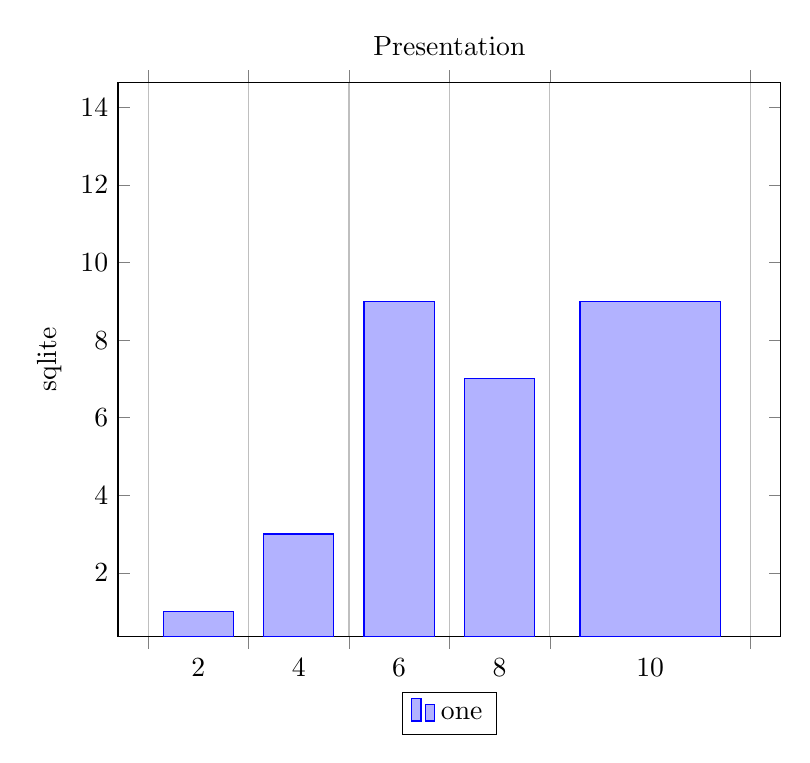
\begin{tikzpicture}
                    \begin{axis}[
                    x tick label style={/pgf/number format/1000 sep=},
                    ylabel=sqlite,
                    xlabel=sql,
                    enlargelimits = 0.050000,
                    legend style={at={(0.500000,-0.100000)},	anchor=north, legend columns=-1},
                    ybar interval=0.700000,
                    title={Presentation}
                    ]
                    \addplot
                          coordinates {
                          (2,1)(4,3)(6,9)(8,7)(10,9)(14,14)
                          };

                    \legend{one}
                    \end{axis}
                    \end{tikzpicture}
											\hskip 5pt

                        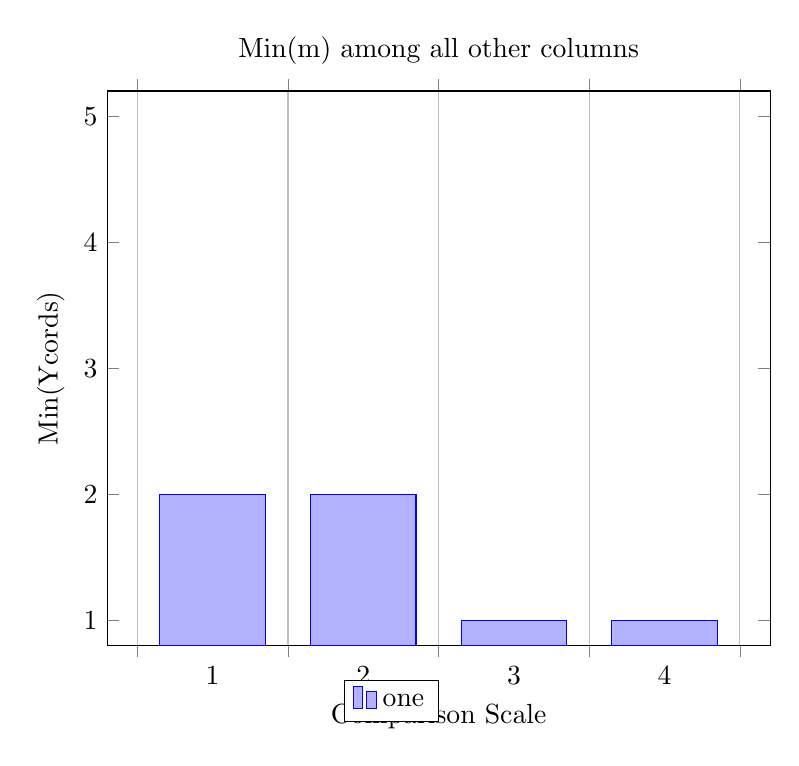
\begin{tikzpicture}
                        \begin{axis}[
                        x tick label style={/pgf/number format/1000 sep=},
                        ylabel=Min(Ycords),
                        xlabel=Comparison Scale,
                        enlargelimits = 0.050000,
                        legend style={at={(0.500000,-0.100000)},	anchor=east, legend columns=-1},
                        ybar interval=0.700000,
                        title={Min(m) among all other columns}
                        ]
                        \addplot
                       coordinates {
                       (1,2)(2,2)(3,1)(4,1)(5,5)
                       };

                        \legend{one}
                        \end{axis}
                        \end{tikzpicture}
\end{document}
